\documentclass[10pt]{article}

\usepackage[margin=1in]{geometry}
\usepackage{float,glossaries,graphicx,hyperref}

\makenoidxglossaries

\newglossaryentry{Binary Separated Value}
{
    name=Binary Separated Value,
    description={The filetype associated with the encoding protocols laid out in this document}
}

\newglossaryentry{.bsvx}
{
    name=.bsvx,
    description={The file extension associated with the Binary Separated Value file format}
}

\newglossaryentry{.csv}
{
    name=.csv,
    description={Comma-separated values file format often used for databases and spreadsheets}
}

\newglossaryentry{.tsv}
{
    name=.tsv,
    description={Tab-separated values file format used for databases and spreadsheets}
}

\newglossaryentry{Comma delimiter}
{
    name=Comma delimiter,
    description={Practice of using the ‘,’ character as a field separator to differentiate records in a file. Instances of a comma are always interpreted as a delimiter unless they appear in doubles quotes e.g. “1,0”}
}

\newglossaryentry{Serialization}
{
    name=Serialization,
    description={The process of encoding an object as a .bsvx format byte stream}
}

\newglossaryentry{Deserialization}
{
    name=Deserialization,
    description={The process of decoding of a .bsvx byte stream and reconstruction of the original data}
}

\newglossaryentry{Libre Calc}
{
    name=Libre Calc,
    description={An open-source application for manipulating spreadsheets. Developed and maintained by The Document Foundation}
}

\begin{document}

\title{Binary Separated Value}
\author{B. Bean, N. Mezher, J. Summers \& D. Toomey\\University of Massachusetts Lowell | Software Engineering II\\Prof. James Daly}
\date{April 2020}
\maketitle

\section*{Motivation}

The use of databases as a means for storing information has become ubiquitous in every field concerning data.
One of the most common methods for analyzing sets of data from databases is to export it to a \texttt{.csv} (comma separated value) file format in order to manipulate the data via a spreadsheet program or language libraries.
But despite all its draws, the \texttt{.csv} format has some significant drawbacks as well.
The format is too bulky and inefficient for many applications, and it relies on a comma delimiter to separate data which can be problematic \cite{Coleman2011}.
Our improvements upon the \texttt{.csv} format allow for users and programs to more efficiently store and utilize complex data.
The end goal is to expedite communication between programs and disparate systems.

\indent{}
This document first outlines a new file format termed Binary Separated Value (BSVX), with the file extension \texttt{.bsvx}.
This is not to be confused with the \texttt{.bsv} file format, which is a BASIC BSave Graphics file.
The tailing \texttt{x} was chosen for convenience as it makes the name of our format, \texttt{.bsvx}, wholly unique.
This format of data is delimited with byte markers which begin each field telling the library what kind of data will be in the field and how long it will be.
Using byte markers, instead of plaintext character delimiters, solves a key issue with the \texttt{.csv} format---strings including commas do not prematurely end a field.
The Binary Separated Value format is processed through a proprietary Python library called \texttt{bsvxpy}.

\indent{}
One drawback of this style of implementation is the inability to parse and edit \texttt{.bsvx} files through a text editor.
However, this issue is remedied through the BSVX LibreOffice Calc Extension.
\href{https://www.libreoffice.org/discover/libreoffice/}{LibreOffice} is a free to use, open-source file editing platform similar to Microsoft Office.
\href{https://www.libreoffice.org/discover/calc/}{Calc} is a program provided in the LibreOffice suite, and provides similar functionality to Microsoft’s Excel program \cite{Guthrie2012}.
The BSVX LibreOffice Calc Extension gives LibreOffice Calc users the ability to read data from \texttt{.bsvx} files and export their spreadsheets to \texttt{.bsvx} files.
Users also have the ability to import, then convert \texttt{.csv} files into \texttt{.bsvx} files through the BSVX LibreOffice Calc Extension.

\section*{BSVX File Format Specification}

Each \texttt{.bsvx} file contains a series of rows of headers or records.
Each row begins with a byte marker denoting the type (i.e. header or record) and the number of fields within that row.
Following the first byte marker of a row is a series of fields, each made up of two parts: a byte marker denoting the type and size of the data stored within the field, and the data itself.
Some initial markers indicate that the size of the data is given in subsequent bytes.
Once the length \textit{n} is determined, those \textit{n} bytes can be interpreted to match the field byte marker.
Each row does not have to be the same length, the data can be jagged and parsers read as much data as is denoted by the first byte marker of each row. 

\indent{}
At any time, the parser knows how many bytes it needs to read.
There is never an instance where the parser needs to read bytes until it sees a particular character (as opposed to \texttt{.csv} or \texttt{.tsv} parsers, which look for commas or tabs respectively).
Strings need neither end marks nor escape characters, and are stored in the UTF-8 format.
The byte marker for strings denotes the number of bytes read, not the number of characters of the string itself.
All numbers are stored in little endian order.

\indent{}
An abstract example of a \texttt{.bsvx} file row (header or record) looks like this:

\begin{table}[H]
\centering
\begin{tabular}{|c|c|c|c|c|c|c|}
\hline
3 & 3 & FOO & 2 & 1000 & 4 & 25.345 \\
Field & str &  & int &  & Float &  \\ \hline
\end{tabular}
\caption{An example of a \texttt{.bsvx} file row.}
\label{tab:bsvxApproach_example}
\end{table}

\indent{}
The same example of a \texttt{.bsvx} file row (header or record) but represented in hexadecimal:

\begin{table}[H]
\centering
\begin{tabular}{|c|c|c|c|c|c|c|}
\hline
0xAB & 0x03 & 0x464F4F & 0x91 & 0x01F4 & 0x9C & 0x400395851EB851EB851EB851EB851EB8 \\
Record & str &  & int &  & Float &  \\ \hline
\end{tabular}
\caption{An example of a \texttt{.bsvx} file row in hex values.}
\label{tab:bsvxApproach_example in hexadecimal}
\end{table}

\indent{}
The following table displays the implementation for each type of supported data in its own class.
Bit ranges for each field are also provided; they are denoted by values ranging from 0 to 255.
The first column gives the parser crucial context: what type of data follows the byte marker, and further, which \textit{variant} on that type it is.
For example, the short integer type is represented by numbers in the range 136-143. 
A 2 byte short integer is indicated by 138, 139 indicates a 3 byte integer, 140 indicates a 4 byte integer, etc.
The second column illustrates how the range of values for a given type is affected by the magnitude of its offset.
I.e. for a short integer, the second column entry is 136 + [0, 7].
The third column establishes the types of data that are supported, and the fourth column provides a brief description of each.

\begin{table}[H]
\centering
\resizebox{\textwidth}{!}{%
\begin{tabular}{|c|c|c|l|}
\hline
\textbf{Range} & \textbf{Form} & \textbf{Name} & \textbf{Description} \\ \hline
0 &  & Blank & Possible implementation: NULL or ‘empty string’ \\ \hline
1-127 & 1-127 & Short str & UTF-8 Encoded string of byte length 1-127 \\ \hline
128-135 & 128 + {[}0,7{]} & Long str & 1-8 bytes giving the length of a str, followed by said str \\ \hline
136-143 & 136 + {[}0,7{]} & Short int & An integer in the range of 0-7 bytes \\ \hline
144-151 & 144 + {[}0,7{]} & Long int & A zig-zag encoded integer using 1-8 bytes \\ \hline
152-159 & 152 + {[}0,7{]} & Float & IEEE-754 format float: 0 = half precision, 1 = single, 2 = double, 3 = triple \\ \hline
160-167 & 160 + {[}0,7{]} & Blob & 1-8 bytes giving the length of binary data in bytes, followed by said data \\ \hline
168-183 & 168 + {[}0,15{]} & Header & Beginning of header with 0-15 fields \\ \hline
184-191 & 184 + {[}0,7{]} & Long header & 1-8 bytes giving the number of fields in the header \\ \hline
192-207 & 192 + {[}0,15{]} & Record & Beginning of record with 0-15 fields \\ \hline
208-215 & 208 + {[}0,7{]} & Long record & 1-8 bytes giving the number of fields in the record \\ \hline
216-255 &  & Reserved & For future use \\ \hline
\end{tabular}%
}
\caption{Data types supported by the BSVX file format specification.}
\label{tab:bsvxApproach_dataTypes}
\end{table}

\section*{Deliverables}

The deliverables for this new file format include the aforementioned BSVX LibreOffice Calc Extension and \texttt{bsvxpy} Python library.
The LibreOffice Calc extension should be capable of ultimately converting between \texttt{.csv} and \texttt{.bsvx} files without loss or adulteration of information.
Similar libraries for languages such as Java, C++, or JavaScript are left as stretch goals.

\indent{}
The BSVX LibreOffice Calc Extension allows spreadsheets to be saved to and read from \texttt{.bsvx} files.
To illustrate the top-most point for user interaction with the BSVX LibreOffice Calc Extension, there is included a series of figures below. 
\autoref{fig:deliverables_mockupPart1} displays the default toolbar packaged with LibreOffice Calc.
\autoref{fig:deliverables_mockupPart2} contrasts the differences between the default toolbar and the toolbar with the BSVX LibreOffice Calc Extension enabled.
It can be seen that only two features are added, in the form of two buttons.
The proposed left button allows for importing, reading from, a \texttt{.bsvx} file and the proposed right button for exporting, saving to, a \texttt{.bsvx} file.
Finally, \autoref{fig:deliverables_mockupPart3} provides a glance as to how the toolbar looks with the BSVX LibreOffice Calc Extension enabled.

\begin{figure}[H]
\centering
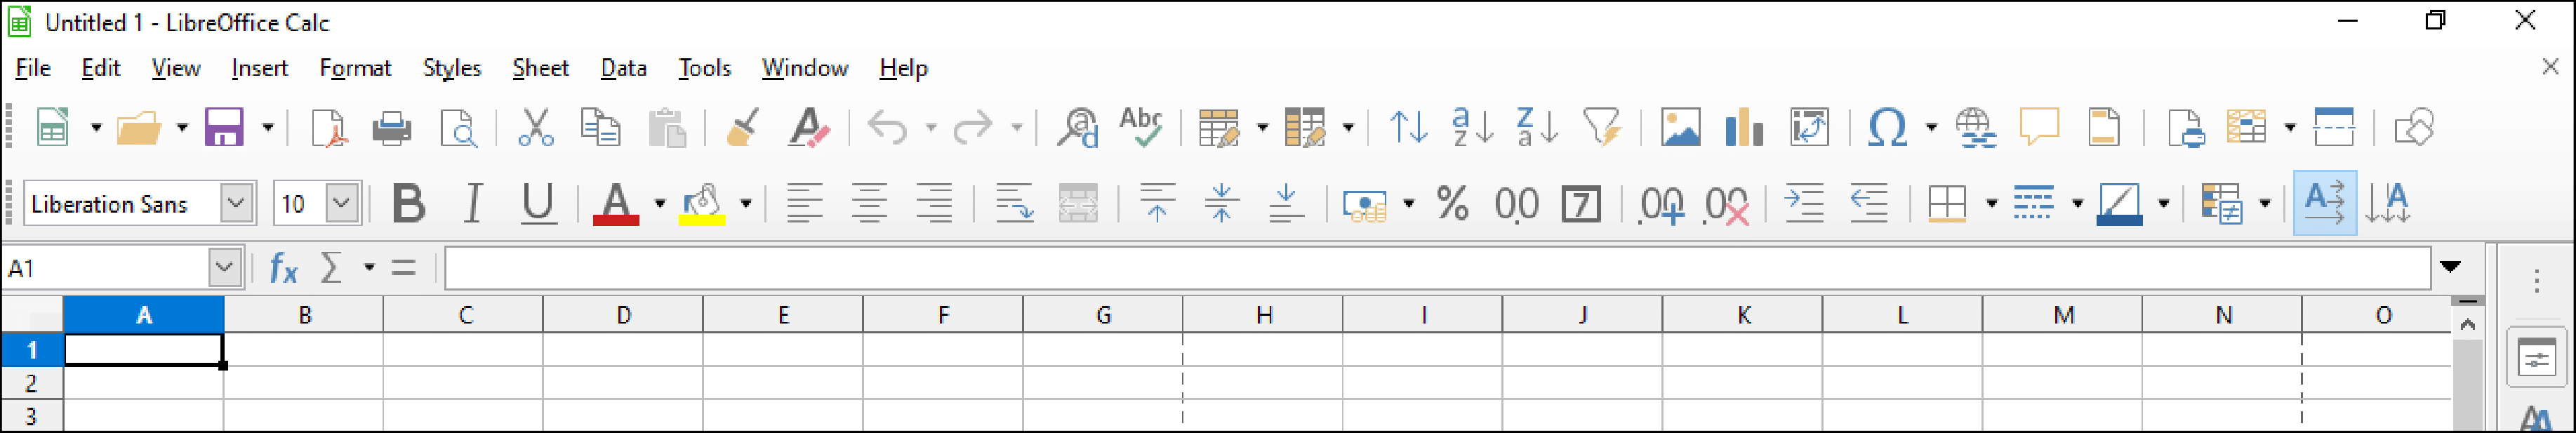
\includegraphics[width=\textwidth]{figures/mockupPart1.png}
\caption{LibreOffice Calc's toolbar.}
\label{fig:deliverables_mockupPart1}
\end{figure}

\begin{figure}[H]
\centering
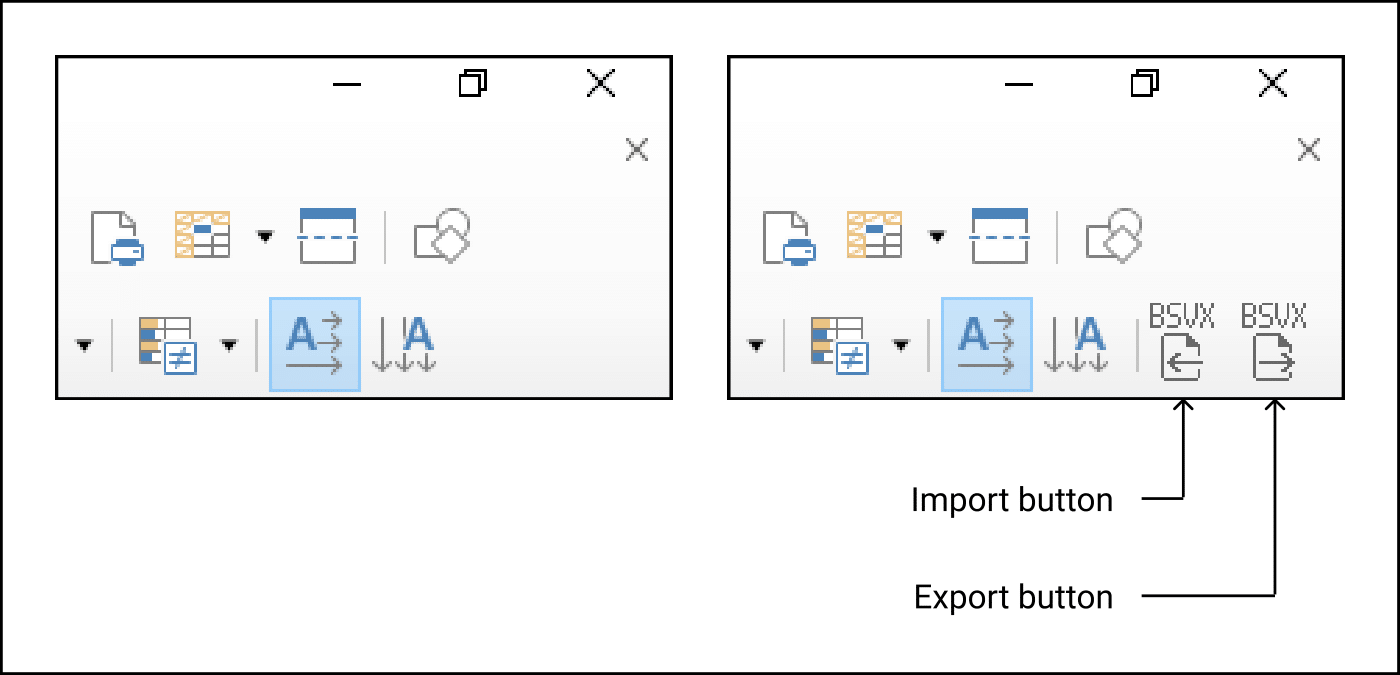
\includegraphics[width=4in]{figures/mockupPart2.png}
\caption{The BSVX LibreOffice Calc Extension provides two additional buttons for importing and exporting.}
\label{fig:deliverables_mockupPart2}
\end{figure}

\begin{figure}[H]
\centering
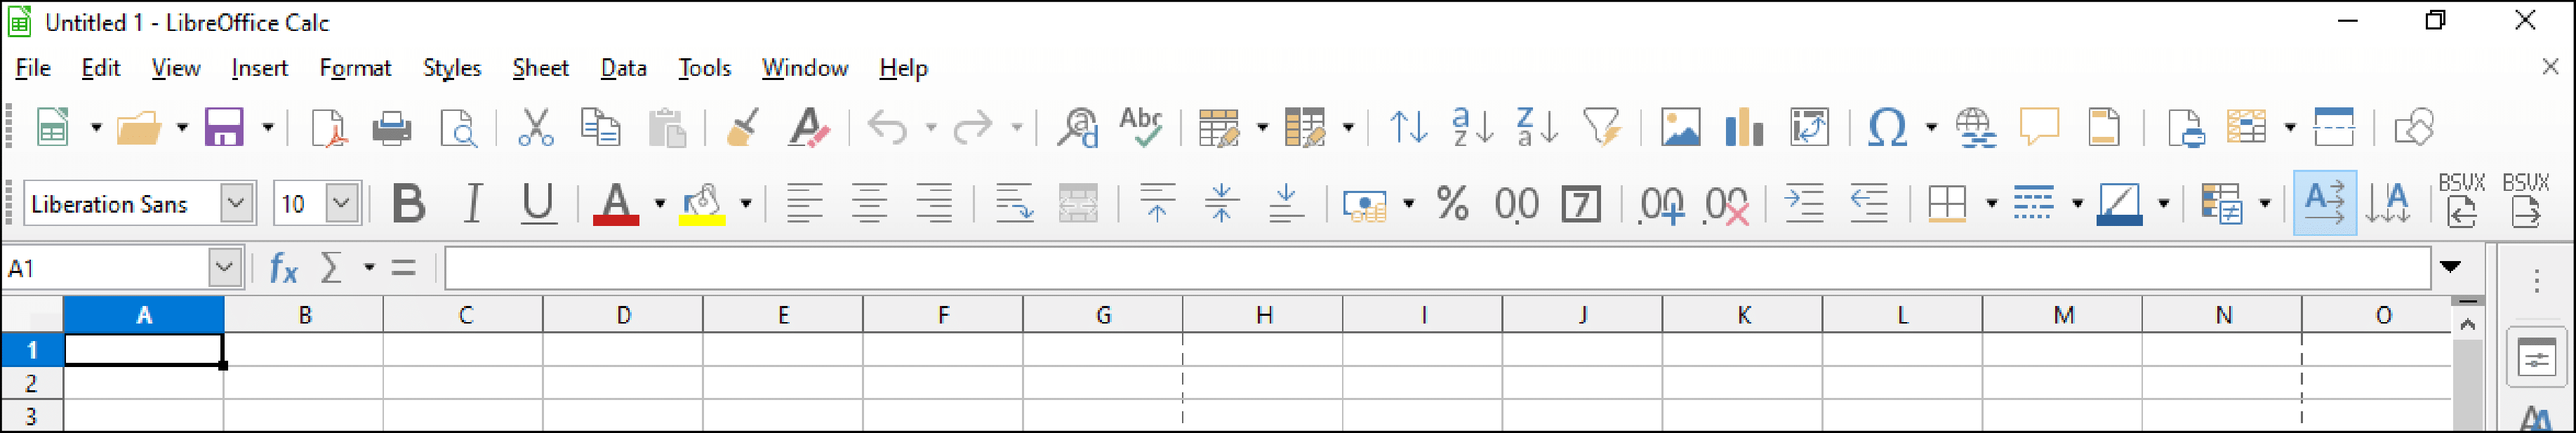
\includegraphics[width=\textwidth]{figures/mockupPart3.png}
\caption{A mockup of LibreOffice Calc's toolbar with the BSVX LibreOffice Calc Extension enabled.}
\label{fig:deliverables_mockupPart3}
\end{figure}

\indent{}
To talk more about how the BSVX LibreOffice Calc Extension works behind the scenes, it is first necessary to speak about our Python library---\texttt{bsvxpy}.
As a generality, our Python library is similar to the \texttt{.csv} Python library.
A writer function is passed a series of fields representing a header row. 
Subsequent binary values are decoded based on the corresponding type casts provided by the header.
The library then extracts each of the fields from the dictionary object and outputs them to the LibreOffice Calc spreadsheet in sequential order.
The library also processes nested data structures within the \texttt{.bsvx} file, allowing for the recursive encoding and decoding of further dictionary objects.

\begin{figure}[H]
\centering
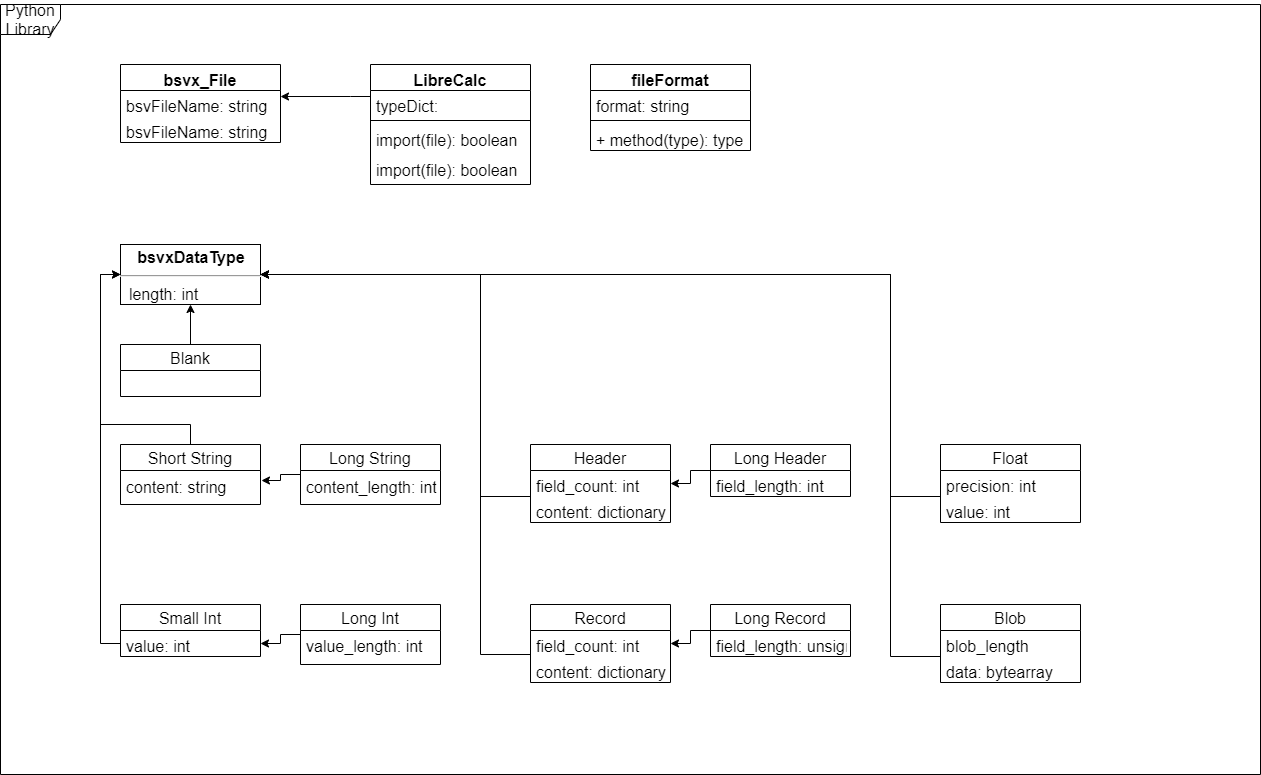
\includegraphics[width=\textwidth]{figures/bsvxpy.png}
\caption{UML diagram outlining the classes and statstructures used in \texttt{bsvxpy}}
\label{fig:bsvxpy_architecture}
\end{figure}

\indent{}
With an understanding of how the \texttt{bsvxpy} Python library functions, we can return to an overview of the BSVX LibreOffice Calc Extension.
First off, the LibreOffice Calc project allows developers to create extensions using Python, which let us extend LibreOffice Calc’s functionality to include \texttt{.bsvx} file format support using our \texttt{bsvxpy} Python library.
We also used the \texttt{uno} Python library, as it is necessary for any LibreOffice Calc extension development.

\indent{}
A novel problem with a strongly typed encoding is the inability to handle undefined data types such as graphs or algorithms that are often used in spreadsheet applications.
To solve this, the \texttt{.bsvx} file format manages unknown data types with a catch-all data type---Blob---which acts as a polymorphic object.
These Blobs store raw binary data imported from spreadsheets or \texttt{.csv} files.
By relying on the raw binary for unknown data types, \texttt{bsvxpy} can accommodate proprietary encodings associated with any third party application.
As a note, this introduces the risk of \texttt{.bsvx} files being limited to one spreadsheet application when using Blob data types.
This is because third party applications may use internal encodings which are unknown to other programs.

\indent{}
To export data to a \texttt{.bsvx} file, the BSVX LibreOffice Calc Extension calls functions from the \texttt{uno} Python library to read cell data from LibreOffice Calc.
The \texttt{bsvxpy} Python library is then used to convert that data into binary separated values.
Once the data is appropriately converted, it is written to a file with the extension \texttt{.bsvx} and as named by the user.
\autoref{fig:deliverables_dataToBsvx} depicts the data flow for the exporting feature.

\begin{figure}[H]
\centering
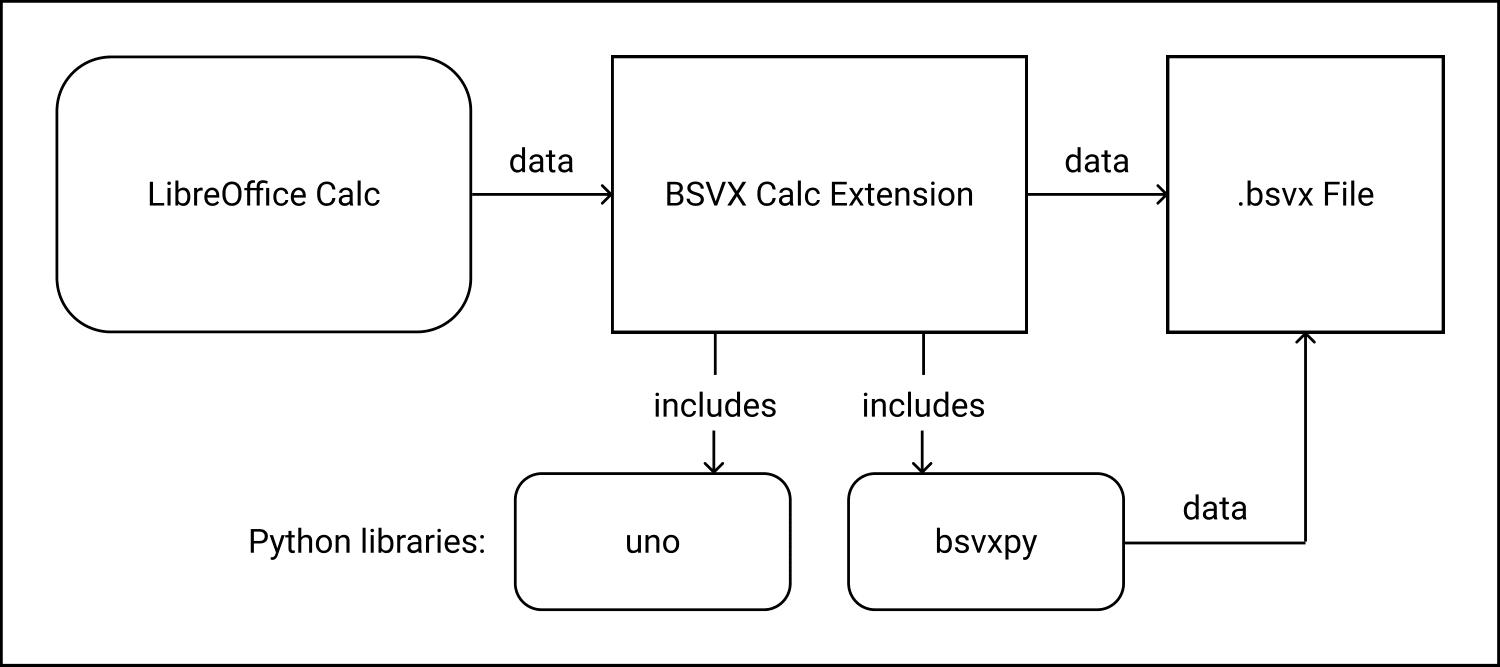
\includegraphics[width=5in]{figures/dataToBsvx.png}
\caption{Scope of API and library calls for the BSVX LibreOffice Calc Extension in exporting data to a \texttt{.bsvx} file.}
\label{fig:deliverables_dataToBsvx}
\end{figure}

\indent{}
The importing feature works the same way, but in reverse.
The user selects a \texttt{.bsvx} file to import data from, and the BSVX LibreOffice Calc Extension reads data from that file, using \texttt{bsvxpy} and \texttt{uno} to translate it from binary separated value data to cell data that LibreOffice Calc can read.
The data flow for the importing feature is represented by \autoref{fig:deliverables_bsvxToData}.
    
\begin{figure}[H]
\centering
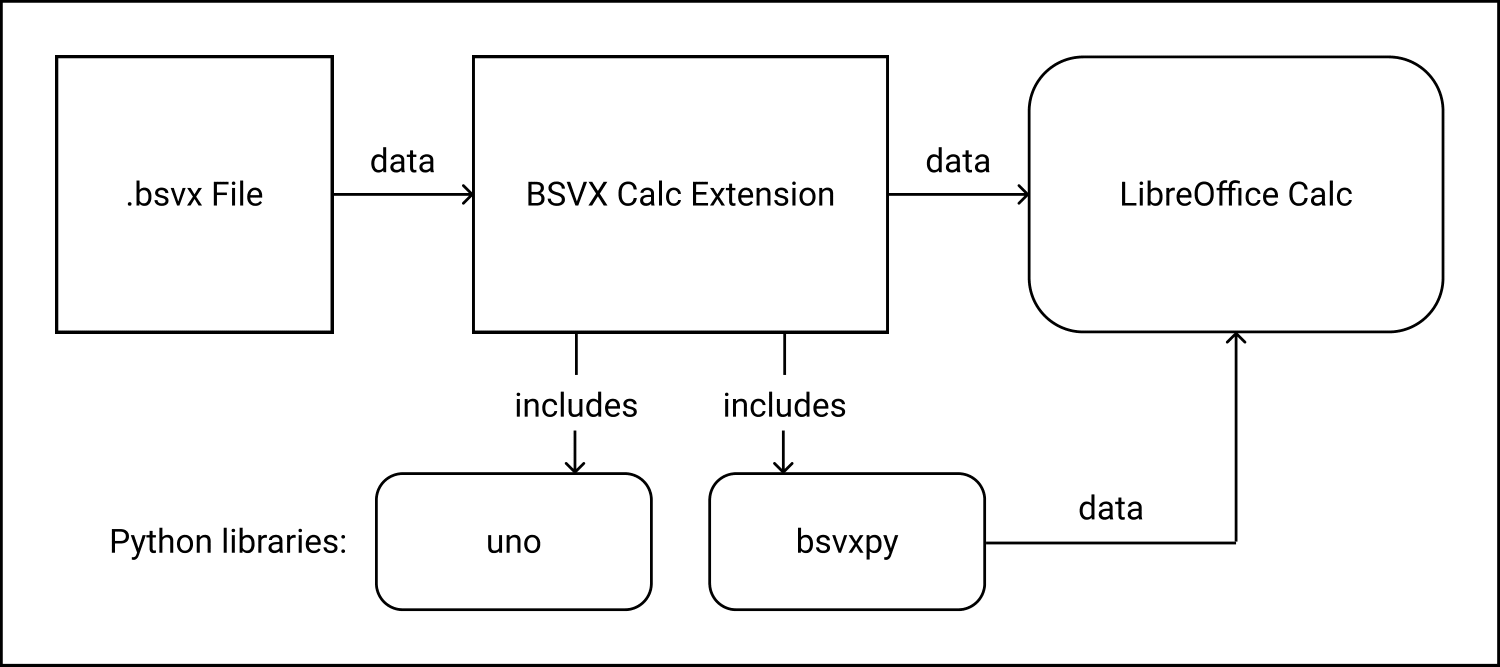
\includegraphics[width=5in]{figures/bsvxToData.png}
\caption{Scope of API and library calls for the BSVX LibreOffice Calc Extension in importing data from a \texttt{.bsvx} file.}
\label{fig:deliverables_bsvxToData}
\end{figure}

\indent{}
This functionality also allows the user to convert from \texttt{.csv} to \texttt{.bsvx}.
If the user chooses to import a \texttt{.csv} file into LibreOffice Calc, and exports that file to a \texttt{.bsvx} file, that same data becomes available in both files.
Likewise, if the user chooses to import a \texttt{.bsvx} file and export that file to a \texttt{.csv} file, that same data becomes available.
These changes do not significantly affect the overall architecture of LibreOffice Calc.
The same base functionality of LibreOffice Calc is still provided to the user once this extension is installed, with the addition of importing and exporting features for the \texttt{.bsvx} format.

\section*{Approach}

As the specifications for the \texttt{.bsvx} format have already been articulated, our main goal was to implement novel importing and exporting functionality in LibreOffice Calc.
Example \texttt{.bsvx} files have been created to accurately account for testing basic functionality as well as edge cases.
Initial builds emphasized basic functionality, such as correctly reading and writing basic data types.
Nested and blob types were handled after initial testing was completed.
In every step of the process, we attempted to optimize memory and computational efficiency to improve our performance outcomes.

\indent{}
One important test of the \texttt{.bsvx} format, and its corresponding extension, was its capacity to maintain full integrity of the data after conversion to and from the \texttt{.csv} format.
A user with minimal experience in LibreOffice and some experience with spreadsheets should be able to perform these conversions without loss of data or corruption of its ordering.
We accepted some loss of formatting and style, provided the order of the values and the values themselves were maintained.

\indent{}
The project was expected to take approximately two months to complete, with production wrapping in late April 2020.
Costs were minimal, if nonexistent, as our developers were paid in “experience.”

\section*{Development}

In developing the \texttt{bsvxpy} Python library, our team took a number of precautions.
At the highest level, our project was split into three different repositories on GitHub, so that BSVX's components were entirely separate.
The \href{https://github.com/bsvx/bsvxpy}{\texttt{bsvxpy} repository} holds our \texttt{bsvxpy} Python library.
The \href{https://github.com/bsvx/bsvx4calc}{\texttt{bsvx4calc} repository} holds our BSVX LibreOffice Calc Extension.
Lastly, the \href{https://github.com/bsvx/docs}{\texttt{docs} repository} contains efforts related to this document and generating the results shown later in this document.

\indent{}
To further isolate BSVX, the development of the \texttt{bsvxpy} Python library required the use of a Python virtual environment.
This ensured that the user did not install the incomplete module on their default Python environment.
Specifics regarding the initialization and launch of a Python virtual environment, within the context of this project, can be found in the README portion of the \href{https://github.com/bsvx/bsvxpy}{\texttt{bsvxpy} repository}.

\indent{}
To ensure correctness, to the best of the BSVX developers, Travis-CI was utilized.
Travis-CI allows for integration with GitHub repositories, and helped to automatically test BSVX's components.
As for the tests themselves, the \texttt{pytest} package was utilized.
The \texttt{pytest} package allowed the BSVX developers to easily and quickly construct unit and systems tests for the \texttt{bsvxpy} Python library.
Different testing files were associated for each data type supported by the BSVX file format specification so that each component's functionality could be tested separated if needed.
If all tests that were tested---typically all tests created---passed, Travis-CI would assign our repository a passing mark.
Failing Travis-CI marks enabled our developers to retroactively fix problems with some context as to where they happened.
This continuous integration process made development safe and incremental.

\section*{Schedule and Milestones}

\begin{table}[H]
\centering
\begin{tabular}{|p{80pt}|p{375pt}|}
\hline
\textbf{Date} & \textbf{Goal} \\ \hline
February 14, 2020 & Finish initial background research, Draft BSV Proposal deliverable. \\ \hline
February 26, 2020 & Finalize project's architecture, draft Project Architecture deliverable\\ \hline
March 4, 2020 & \textbf{Midterm Milestone:} Present progress and evaluate stretch goals \\ \hline
March 18, 2020 & Implement csv/bsvx backend\\ \hline
April 1, 2020 & Draft the Initial Results deliverable \\ \hline
April 27, 2020& \textbf{Final Milestone:} Submit Final Report and Present findings to class \\ \hline
\end{tabular}
\caption{A schedule of our project's events.}
\label{tab:approach_schedule}
\end{table}

\section*{Challenges and Risks}

One of the primary risks was the possibility that there were undiscovered ambiguities in the format specification.
These were dealt with by tightening the specification to account for ambiguities, and updating the reference implementation.
Additionally, parsing \texttt{.csv} files for conversion to \texttt{.bsvx} files, and vice-versa, involved numerous pitfalls.
While there was an agreed upon standard format for \texttt{.csv} files, it didn’t come about until 2005 and many \texttt{.csv} files still did not conform to it strictly.
This complicated our attempt to ensure integrity and continuity between conversions for \textit{all} \texttt{.csv} and \texttt{.bsvx} files.
For instance, when converting a \texttt{.bsvx} file consisting of several strings of comma characters, our library had to ensure that none of the commas ended up being misinterpreted as delimiters.
Properly following the specification ensured consistency and prevented this from happening, but rigorous testing with a myriad of files was necessary.

\indent{}
One challenge fundamental to the \texttt{.bsvx} format itself was deciding how to handle Blob objects.
It is not always clear what type of data a Blob should be deserialized as.
We took the stance that the user should have context of the Blob's contents, so anything outside of the confines of the BSVX specification is not BSVX's responsibility.
LibreOffice Calc may contain methods to interpret unknown fields upon reading the file but more research on this is necessary.
Another challenge was that the framework/API for both LibreOffice and LibreOffice Calc was unfamiliar to our developers; it took them some time to learn how to engage with LibreOffice Calc.

\section*{Results}

In diagnosing the successfulness of our project and of BSVX's subcomponents themselves, we created a script that generates a number of key figures.
This script can be found in the scripts folder of our \href{https://github.com/bsvx/docs}{\texttt{docs} repository} along with usage instructions in the form of a README.
We offer this means of figure self-generation such that it is clear and self-provable that all figures in this document are fair.

\indent{}
An aspect integral to BSVX is the compression of information attained through storing fields in hexadecimal.
In comparing relative sizes of equivalent \texttt{.csv} and \texttt{.bsvx} files, it is demonstrably clear that \texttt{.bsvx} files are smaller in file weight.

\begin{figure}[H]
\centering
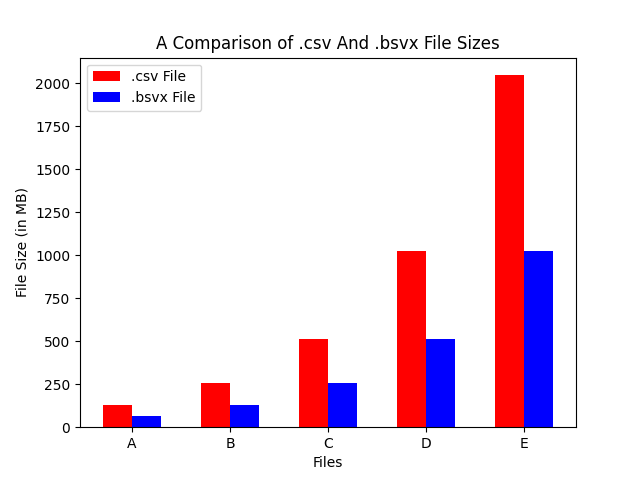
\includegraphics[width=5in]{scripts/figures/1.png}
\caption{A simplified version of a graphic that will be in the final version of our report.}
\label{fig:results_1}
\end{figure}

\indent{}
Comma delimiter issues are another problem BSVX sought to solve.
Displayed below is a graph of expected versus actual fields for equivalent \texttt{.csv} and \texttt{.bsvx} files.
\texttt{.bsvx} files match the expected number of fields, whereas \texttt{.csv} files decidedly do not.
In fact, \texttt{.csv} files develop an increasingly larger margin of error with larger file sizes.

\begin{figure}[H]
\centering
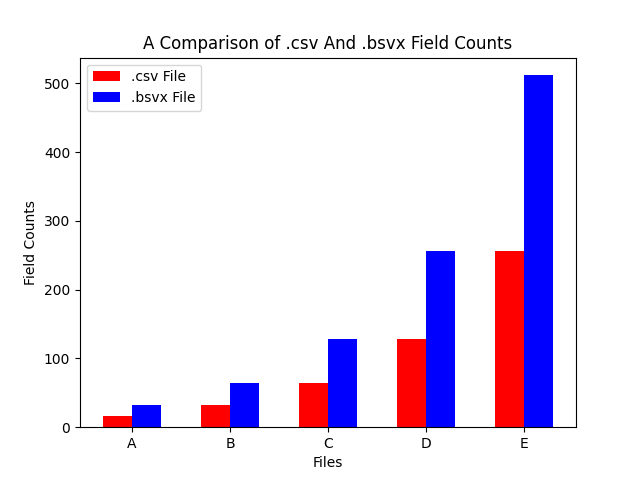
\includegraphics[width=5in]{scripts/figures/2.png}
\caption{A simplified version of a graphic that will be in the final version of our report.}
\label{fig:results_2}
\end{figure}

\indent{}
From here we can see that the two main problems with \texttt{.csv} files, as previously noted, have been solved with our implementation of the BSVX file format specification.

\clearpage
\glsadd{Binary Separated Value}
\glsadd{.bsvx}
\glsadd{.csv}
\glsadd{.tsv}
\glsadd{Comma delimiter}
\glsadd{Serialization}
\glsadd{Deserialization}
\glsadd{Libre Calc}
\printnoidxglossary[nonumberlist]

\clearpage
\begin{thebibliography}{9}

  \bibitem{Coleman2011}
    Coleman, Larry.
    "Why do we keep using CSV?"
    Software Engineering Stack Exchange,
    14 Feb. 2011.
    \url{https://softwareengineering.stackexchange.com/questions/47838/why-do-we-keep-using-csv}

  \bibitem{"CSV File Reading and Writing"2020}
    “CSV File Reading and Writing.”
    Python Docs,
    12 Feb. 2020.
    \url{https://docs.python.org/3/library/csv.html}

  \bibitem{DalyMeiners2020}
    Daly, James and Meiners, Chad.
    “Binary Separated Value.”
    UMass Lowell,
    30 Jan. 2020.

  \bibitem{Guthrie2012}
    Guthrie, Gordon.
    “How to Work With LibreOffice Calc.”
    TechRadar,
    23 July 2012.
    \url{https://www.techradar.com/news/world-of-tech/roundup/how-to-work-with-libreoffice-calc-1089870}
  
\end{thebibliography}

\end{document}
